\chapter{Special functions in genr}
\label{chap-genr}

\section{Introduction}
\label{genr-intro}

The \cmd{genr} command provides a flexible means of defining new
variables.  It is documented in the \GCR.  This chapter offers a more
expansive discussion of some of the special functions available via
\verb+genr+ and some of the finer points of the command.
    
\section{Long-run variance}
\label{sec:lrvar}

As is well known, the variance of the average of $T$ random variables
$x_1, x_2, \ldots, x_T$ with equal variance $\sigma^2$ equals
$\sigma^2/T$ if the data are uncorrelated. In this case, the sample
variance of $x_t$ over the sample size provides a consistent estimator.

If, however, there is serial correlation among the $x_t$s, the
variance of $\bar{X} = T^{-1} \sum_{t=1}^T x_t$ must be estimated
differently. One of the most widely used statistics for this purpose
is a nonparametric kernel estimator with the Bartlett kernel defined
as
\begin{equation}
  \label{eq:scalar-lrvar}
  \hat{\omega}^2(k) = T^{-1} \sum_{t=k}^{T-k} \left[ \sum_{i=-k}^k w_i (x_t -
  \bar{X}) (x_{t-i} - \bar{X}) \right] ,
\end{equation}
where the integer $k$ is known as the window size and the $w_i$ terms
are the so-called \emph{Bartlett weights}, defined as $w_i = 1 -
\frac{|i|}{k + 1}$. It can be shown that, for $k$ large enough,
$\hat{\omega}^2(k)/T$ yields a consistent estimator of the variance of
$\bar{X}$.

\app{Gretl} implements this estimator by means of the function
\texttt{lrvar()}, which takes two arguments: the series whose long-run
variance must be estimated and the scalar $k$. If $k$ is negative, the
popular choice $T^{1/3}$ is used.

\section{Cumulative densities and p-values}
\label{sec:genr-cdf}

The two functions \cmd{cdf} and \cmd{pvalue} provide complementary
means of examining values from several probability distributions: the
standard normal, Student's $t$, $\chi^2$, $F$, gamma, and binomial.
The syntax of these functions is set out in the \GCR; here we expand
on some subtleties.

The cumulative density function or CDF for a random variable
is the integral of the variable's density from its lower limit
(typically either $-\infty$ or 0) to any specified value $x$.  The
p-value (at least the one-tailed, right-hand p-value as returned by
the \cmd{pvalue} function) is the complementary probability, the
integral from $x$ to the upper limit of the distribution, typically
$+\infty$.  

In principle, therefore, there is no need for two distinct functions:
given a CDF value $p_0$ you could easily find the corresponding
p-value as $1-p_0$ (or vice versa).  In practice, with
finite-precision computer arithmetic, the two functions are not
redundant.  This requires a little explanation.  In \app{gretl}, as in
most statistical programs, floating point numbers are represented as
``doubles'' --- double-precision values that typically have a storage
size of eight bytes or 64 bits.  Since there are only so many bits
available, only so many floating-point numbers can be represented:
\textit{doubles do not model the real line}.  Typically doubles can
represent numbers over the range (roughly) $\pm 1.7977 \times
10^{308}$, but only to about 15 digits of precision.

Suppose you're interested in the left tail of the $\chi^2$ distribution
with 50 degrees of freedom: you'd like to know the CDF value for $x =
0.9$.  Take a look at the following interactive session: 
\begin{code}
? genr p1 = cdf(X, 50, 0.9)
Generated scalar p1 (ID 2) = 8.94977e-35
? genr p2 = pvalue(X, 50, 0.9)
Generated scalar p2 (ID 3) = 1
? genr test = 1 - p2
Generated scalar test (ID 4) = 0
\end{code}

The \cmd{cdf} function has produced an accurate value, but the
\cmd{pvalue} function gives an answer of 1, from which it is not
possible to retrieve the answer to the CDF question.  This may seem
surprising at first, but consider: if the value of \texttt{p1} above
is correct, then the correct value for \texttt{p2} is $1 - 8.94977
\times 10^{-35}$.  But there's no way that value can be represented as
a double: that would require over 30 digits of precision.

Of course this is an extreme example.  If the $x$ in question is not
too far off into one or other tail of the distribution, the \cmd{cdf}
and \cmd{pvalue} functions will in fact produce complementary
answers, as shown below:
\begin{code}
? genr p1 = cdf(X, 50, 30)
Generated scalar p1 (ID 2) = 0.0111648
? genr p2 = pvalue(X, 50, 30)
Generated scalar p2 (ID 3) = 0.988835
? genr test = 1 - p2
Generated scalar test (ID 4) = 0.0111648
\end{code}
But the moral is that if you want to examine extreme values
you should be careful in selecting the function you need, in the
knowledge that values very close to zero can be represented as doubles
while values very close to 1 cannot.


\section{Retrieving internal variables}
\label{sec:genr-internal}

The \cmd{genr} command provides a means of retrieving various values
calculated by the program in the course of estimating models or
testing hypotheses.  The variables that can be retrieved in this way
are listed in the \GCR; here we say a bit more about the special
variables \dollar{test} and \dollar{pvalue}.

These variables hold, respectively, the value of the last test
statistic calculated using an explicit testing command and the p-value
for that test statistic.  If no such test has been performed at the
time when these variables are referenced, they will produce the
missing value code.  The ``explicit testing commands'' that work in
this way are as follows: \cmd{add} (joint test for the significance of
variables added to a model); \cmd{adf} (Augmented Dickey--Fuller test,
see below); \cmd{arch} (test for ARCH); \cmd{chow} (Chow test for a
structural break); \cmd{coeffsum} (test for the sum of specified
coefficients); \cmd{cusum} (the Harvey--Collier $t$-statistic);
\cmd{kpss} (KPSS stationarity test, no p-value available);
\cmd{lmtest} (see below); \cmd{meantest} (test for difference of
means); \cmd{omit} (joint test for the significance of variables
omitted from a model); \cmd{reset} (Ramsey's RESET); \cmd{restrict}
(general linear restriction); \cmd{runs} (runs test for randomness);
\cmd{testuhat} (test for normality of residual); and \cmd{vartest}
(test for difference of variances). In most cases both a \dollar{test}
and a \dollar{pvalue} are stored; the exception is the KPSS test, for
which a p-value is not currently available.
    
An important point to notice about this mechanism is that the internal
variables \dollar{test} and \dollar{pvalue} are over-written each time
one of the tests listed above is performed.  If you want to reference
these values, you must do so at the correct point in the sequence of
\app{gretl} commands.  

A related point is that some of the test commands generate, by
default, more than one test statistic and p-value; in these cases only
the last values are stored. To get proper control over the retrieval
of values via \dollar{test} and \dollar{pvalue} you should formulate
the test command in such a way that the result is unambiguous.  This
comment applies in particular to the \cmd{adf} and \cmd{lmtest}
commands.

\begin{itemize}
\item By default, the \cmd{adf} command generates three variants of
  the Dickey--Fuller test: one based on a regression including a
  constant, one using a constant and linear trend, and one using a
  constant and a quadratic trend.  When you wish to reference
  \dollar{test} or \dollar{pvalue} in connection with this command, you
  can control the variant that is recorded by using one of the flags
  \option{nc}, \option{c}, \option{ct} or \option{ctt} with
  \verb+adf+.
\item By default, the \cmd{lmtest} command (which must follow an OLS
  regression) performs several diagnostic tests on the regression in
  question.  To control what is recorded in \dollar{test} and
  \dollar{pvalue} you should limit the test using one of the flags
  \option{logs}, \option{autocorr}, \option{squares} or
  \option{white}.
\end{itemize}

As an aid in working with values retrieved using \dollar{test} and
\dollar{pvalue}, the nature of the test to which these values relate is
written into the descriptive label for the generated variable.  You
can read the label for the variable using the \cmd{label} command
(with just one argument, the name of the variable), to check that you
have retrieved the right value.  The following interactive session
illustrates this point.

\begin{code}
? adf 4 x1 --c
Augmented Dickey-Fuller tests, order 4, for x1
sample size 59
unit-root null hypothesis: a = 1
  test with constant
  model: (1 - L)y = b0 + (a-1)*y(-1) + ... + e
  estimated value of (a - 1): -0.216889
  test statistic: t = -1.83491
  asymptotic p-value 0.3638
P-values based on MacKinnon (JAE, 1996)
? genr pv = $pvalue
Generated scalar pv (ID 13) = 0.363844
? label pv    
  pv=Dickey-Fuller pvalue (scalar)
\end{code}
%$

\section{The discrete Fourier transform}
\label{sec:genr-fft}

The discrete Fourier transform can be best thought of as a linear,
invertible transform of a complex vector. Hence, if $\mathbf{x}$ is an
$n$-dimensional vector whose $k$-th element is $x_k = a_k + i b_k$,
then the output of the discrete Fourier transform is a vector
$\mathbf{f} = \mathcal{F}(\mathbf{x})$ whose $k$-th element is
\[
  f_k = \sum_{j=0}^{n-1} e^{-i \omega(j,k) } x_j 
\]
where $\omega(j,k) = 2 \pi i \frac{j k}{n}$. Since the transformation
is invertible, the vector $\mathbf{x}$ can be recovered from
$\mathbf{f}$ via the so-called inverse transform
\[
  x_k = \frac{1}{n} \sum_{j=0}^{n-1} e^{i \omega(j,k) } f_j .
\]

The Fourier transform is used in many diverse situations
on account of this key property: the convolution of two vectors can be
performed efficiently by multiplying the elements of their Fourier
transforms and inverting the result.  If
\[
  z_k = \sum_{j=1}^n x_j y_{k-j} ,
\]
then
\[
  \mathcal{F}(\mathbf{z}) = \mathcal{F}(\mathbf{x}) \odot
  \mathcal{F}(\mathbf{y}) .
\]
That is, $\mathcal{F}(\mathbf{z})_k = \mathcal{F}(\mathbf{x})_k
\mathcal{F}(\mathbf{y})_k$.

For computing the Fourier transform, \app{gretl} uses the external
library \texttt{fftw3}: see \cite{frigo05}. This guarantees
extreme speed and accuracy. In fact, the CPU time needed to perform
the transform is $O(n \log n)$ for any $n$. This is why the array of
numerical techniques employed in \texttt{fftw3} is commonly known as
the \emph{Fast} Fourier Transform.

\app{Gretl} provides two matrix functions\footnote{See chapter
  \ref{chap:matrices}.} for performing the Fourier transform and its
inverse: \texttt{fft} and \texttt{ffti}. In fact, \app{gretl}'s
implementation of the Fourier transform is somewhat more specialized:
the input to the \texttt{fft} function is understood to be real.
Conversely, \texttt{ffti} takes a complex argument and delivers a real
result. For example:
\begin{code}
x1 = { 1 ; 2 ; 3 }
# perform the transform
f = fft(a)
# perform the inverse transform
x2 = ffti(f)
\end{code}
yields
\[
  x_1 = \left[ \begin{array}{c} 1 \\ 2 \\ 3 \end{array} \right] 
  \qquad
  f = \left[ \begin{array}{rr} 
      6 & 0 \\ -1.5 & 0.866 \\ -1.5 & -0.866 
   \end{array} \right] 
  \qquad
  x_2 = \left[ \begin{array}{c} 1 \\ 2 \\ 3 \end{array} \right] 
\]
where the first column of \emph{f} holds the real part and the second
holds the complex part. In general, if the input to \texttt{fft} has
$n$ columns, the output has $2n$ columns, where the real parts are
stored in the odd columns and the complex parts in the even
ones. Should it be necessary to compute the Fourier transform on
several vectors with the same number of elements, it is numerically more
efficient to group them into a matrix rather than invoking
\texttt{fft} for each vector separately.

As an example, consider the multiplication of two polynomials:
\begin{eqnarray*}
  a(x) & = & 1 + 0.5 x \\
  b(x) & = & 1 + 0.3 x - 0.8 x^2 \\
  c(x) = a(x) \cdot b(x) & = & 1 + 0.8 x - 0.65 x^2 - 0.4 x^3
\end{eqnarray*}
The coefficients of the polynomial $c(x)$ are the convolution of the
coefficients of $a(x)$ and $b(x)$; the following \app{gretl} code fragment
illustrates how to compute the coefficients of $c(x)$:
\begin{code}
# define the two polynomials
a = { 1, 0.5, 0, 0 }'
b = { 1, 0.3, -0.8, 0 }'
# perform the transforms
fa = fft(a)
fb = fft(b)
# complex-multiply the two transforms 
fc = cmult(fa, fb)
# compute the coefficients of c via the inverse transform
c = ffti(fc)
\end{code}

Maximum efficiency would have been achieved by grouping \texttt{a} and
\texttt{b} into a matrix.  The computational advantage is so little in
this case that the exercise is a bit silly, but the following
alternative may be preferable for a large number of
rows/columns:
\begin{code}
# define the two polynomials
a = { 1 ; 0.5; 0 ; 0 }
b = { 1 ; 0.3 ; -0.8 ; 0 }
# perform the transforms jointly
f = fft(a ~ b)
# complex-multiply the two transforms 
fc = cmult(f[,1:2], f[,3:4])
# compute the coefficients of c via the inverse transform
c = ffti(fc)
\end{code}

Traditionally, the Fourier transform in econometrics has been mostly
used in time-series analysis, the periodogram being the best known
example. Example script \ref{scr:pergm-fft} shows how to compute the
periodogram of a time series via the \texttt{fft} function.

\begin{script}[htbp]
  \caption{Periodogram via the Fourier transform}
  \label{scr:pergm-fft}
\begin{scode}
nulldata 50
# generate an AR(1) process
series e = normal()
series x = 0
x = 0.9*x(-1) + e
# compute the periodogram
scale = 2*pi*$nobs
X = { x }
F = fft(X)
S = sumr(F.^2)
S = S[2:($nobs/2)+1]/scale
omega = seq(1,($nobs/2))' .* (2*pi/$nobs)
omega = omega ~ S
# compare the built-in command
pergm x  
print omega
\end{scode}
\end{script}

\section{The Nadaraya-Watson estimator}
\label{sec:genr-nadarwat}

The Nadaraya-Watson nonparametric estimator is an estimator for the
conditional mean of a variable $Y$, available in a sample of size $n$,
for a given value of a conditioning variable $X$, and is defined as
\[
  m(X) = \frac{ \sum_{j=1}^{n} y_j \cdot K_h(X - x_j)} {\sum_{j=1}^{n} K_h(X - x_j)}
\]
where $K_h(\cdot)$ is the so-called \emph{kernel function}, which is
usually some simple transform of a density function that depends on a
scalar called the \emph{bandwidth}. The one \app{gretl} uses is given
by
\[
  K_h(x) = \exp\left(-\frac{x^2}{2h}\right)
\]
for $|x| < \tau$ and zero otherwise. The scalar $\tau$ is used to
prevent numerical problems when the kernel function is evaluated too
far away from zero and is called the trim parameter.

\begin{script}[htbp]
  \caption{Nadaraya-Watson example}
  \label{scr:nadarwat-ex}
\begin{scode}
# Nonparametric regression example: husband's age on wife's age
open mroz87.gdt

# initial value for the bandwidth
scalar h = $nobs^(-0.2)
# three increasingly smoother estimates
series m0 = nadarwat(HA, WA, h)
series m1 = nadarwat(HA, WA, h * 5)
series m2 = nadarwat(HA, WA, h * 10)

# produce the graph
dataset sortby WA
gnuplot m0 m1 m2 HA WA --output=display --with-lines
\end{scode}
%$
\end{script}

\begin{figure}[htbp]
  \centering
  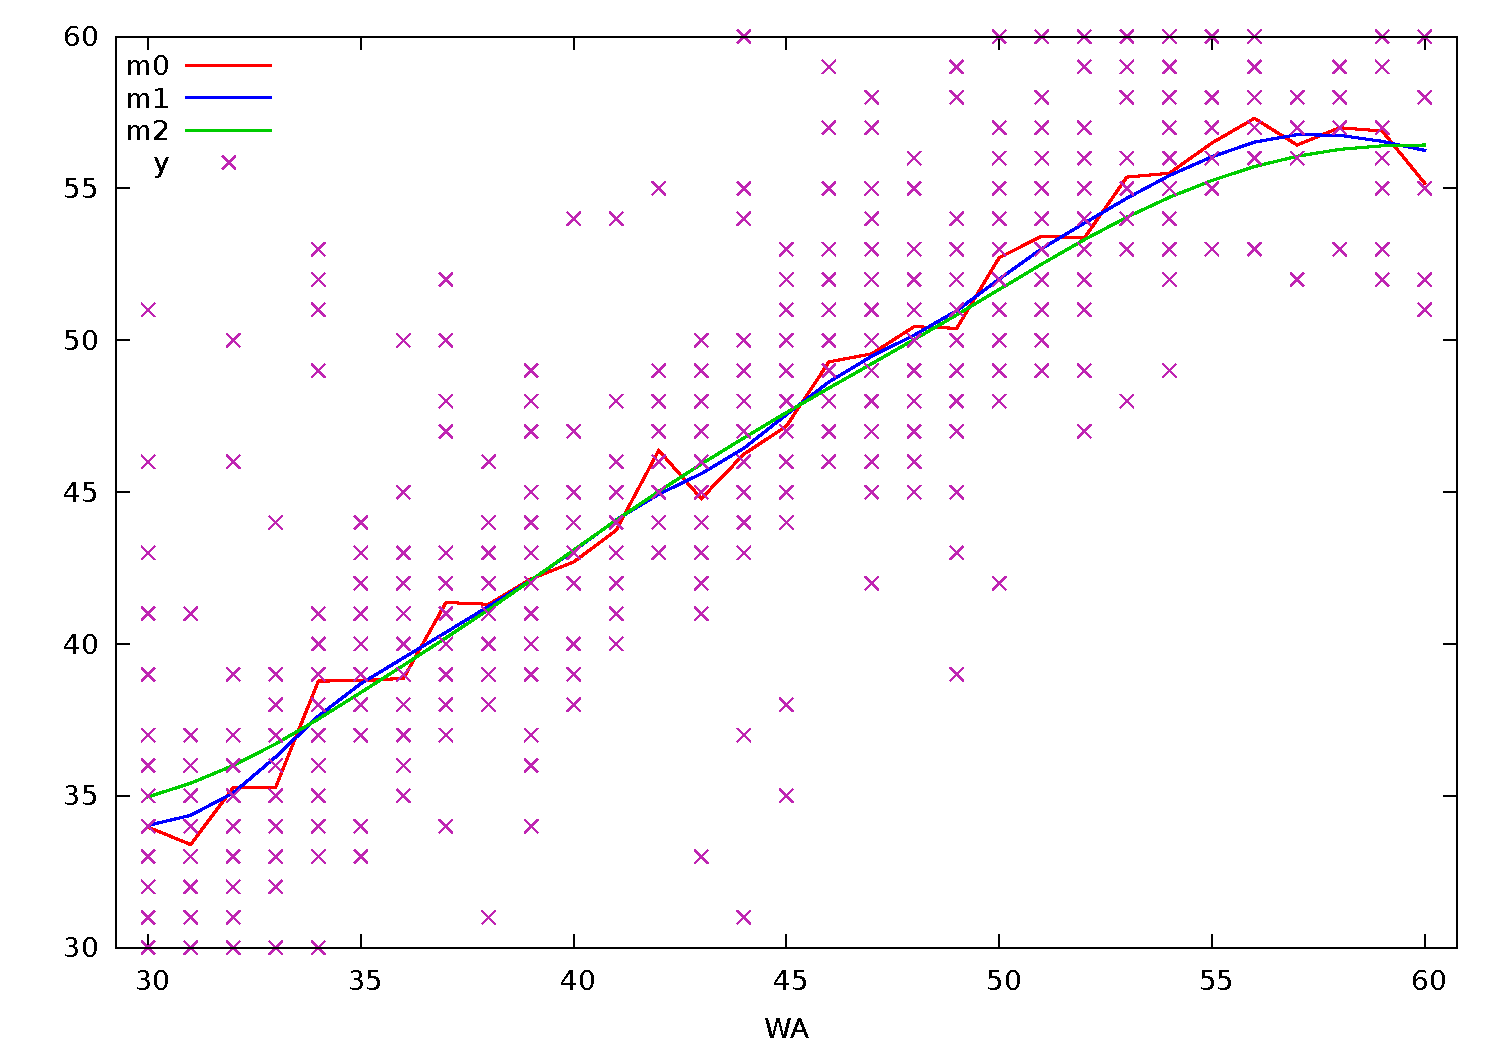
\includegraphics[scale=0.5]{figures/nadarwat-ex}
  \caption{Nadaraya-Watson example for several choices of the bandwidth parameter}
  \label{fig:nadarwat-ex}
\end{figure}

Example script \ref{scr:pergm-fft} produces the graph shown in Figure
\ref{fig:nadarwat-ex} (after some slight editing).

The choice of the bandwidth is up to the user: larger values of $h$
lead to a smoother $m(\cdot)$ function; smaller values make the
$m(\cdot)$ function follow the $y_i$ values more closely, so that the
function appears more ``jagged''. In fact, as $h \to \infty$, $m(x_i)
\to \bar{Y}$; on the contrary, if $h \to 0$, observations for which
$x_i \ne X$ are not taken into account at all when computing $m(X)$.

Also, the statistical properties of $m(\cdot)$ vary with $h$: its
variance can be shown to be decreasing in $h$, while its squared bias
is increasing in $h$.  It can be shown that choosing $h \sim n^{-1/5}$
minimizes the RMSE, so that value is customarily taken as a reference
point.

Note that the kernel function has its tails ``trimmed''. The scalar
$\tau$, which controls the level at which trimming occurs is set by
default at $4 \cdot h$; this setting, however, may be changed via the
\cmd{set} command. For example,
\begin{code}
  set nadarwat_trim 10
\end{code}
sets $\tau = 10 \cdot h$. This may at times produce more sensible
results in regions of $X$ with sparse support; however, you should be
aware that in those same cases machine precision (division by
numerical zero) may render your results spurious. The default is
relatively safe, but experimenting with larger values may be a sensible
strategy in some cases.

A common variant of the Nadaraya-Watson estimator is the so-called
``leave-one-out'' estimator: this is a variant of the estimator that
does not use the $i$-th observation for evaluating $m(x_i)$. This
makes the Nadaraya-Watson estimator more robust numerically and its
usage is often advised for inference purposes.  In formulae, the
leave-one-out estimator is
\[
m(x_i) = \frac{ \sum_{j \ne i} y_j \cdot K_h(x_i -
  x_j)} {\sum_{j \ne i} K_h(x_i - x_j)}
\]
In order to have \app{gretl} compute the leave-one-out estimator, just
reverse the sign of $h$: if we changed example \ref{scr:nadarwat-ex} by
substituting
\begin{code}
  scalar h = $nobs^(-0.2)
\end{code}
with
\begin{code}
  scalar h = -($nobs^(-0.2))
\end{code}
the rest of the example would have stayed unchanged, the only
difference being the usage of the leave-one-out estimator.

Although $X$ could be, in principle, any value, in the typical usage
of this estimator you want to compute $m(X)$ for $X$ equal to one or
more values actually observed in your sample, that is $m(x_i)$. If you
need a point estimate of $m(X)$ for some value of $X$ which is not
present among the valid observations of your dependent variable, you
may want to add some ``fake'' observations to your dataset in which
$y$ is missing and $x$ contains the values you want $m(x)$ evaluated
at. For example, the following script evaluates $m(x)$ at regular
intervals between -2.0 and 2.0:

\begin{code}
nulldata 120
set seed 120496

# first part of the sample: actual data
smpl 1 100
x = normal()
y = x^2 + sin(x) + normal()

# second part of the sample: fake x data
smpl 101 120
x = (obs-110) / 5

# compute the Nadaraya-Watson estimate
# with bandwidth equal to 0.4 (note that
# 100^(-0.2) = 0.398)
smpl full
m = nadarwat(y, x, 0.4)

# show m(x) for the fake x values only
smpl 101 120
print x m -o
\end{code}

and running it produces
\begin{code}
               x            m

101         -1.8     1.165934
102         -1.6     0.730221
103         -1.4     0.314705
104         -1.2     0.026057
105         -1.0    -0.131999
106         -0.8    -0.215445
107         -0.6    -0.269257
108         -0.4    -0.304451
109         -0.2    -0.306448
110          0.0    -0.238766
111          0.2    -0.038837
112          0.4     0.354660
113          0.6     0.908178
114          0.8     1.485178
115          1.0     2.000003
116          1.2     2.460100
117          1.4     2.905176
118          1.6     3.380874
119          1.8     3.927682
120          2.0     4.538364
\end{code}


%%% Local Variables: 
%%% mode: latex
%%% TeX-master: "gretl-guide"
%%% End: 

